%% LyX 2.3.1 created this file.  For more info, see http://www.lyx.org/.
%% Do not edit unless you really know what you are doing.
\documentclass[12pt,english,letterpaper]{kuthesis}
\usepackage{mathptmx}
\renewcommand{\sfdefault}{lmss}
\renewcommand{\ttdefault}{lmtt}
\usepackage[T1]{fontenc}
\usepackage[utf8]{inputenc}
\usepackage{geometry}
\geometry{verbose,tmargin=1in,bmargin=1in,lmargin=1in,rmargin=1in}
\setcounter{secnumdepth}{3}
\setcounter{tocdepth}{3}
\usepackage{color}
\usepackage{tabularx}
\renewcommand*{\arraystretch}{1.4}
\usepackage{babel}
\usepackage{url}
\usepackage{graphicx}
\usepackage{setspace}
\usepackage{esint}
\usepackage[colorinlistoftodos,prependcaption,textsize=tiny]{todonotes}
\usepackage[authoryear]{natbib}
\doublespacing
\usepackage[unicode=true,
 bookmarks=true,bookmarksnumbered=false,bookmarksopen=false,
 breaklinks=true,pdfborder={0 0 0},pdfborderstyle={},backref=false,colorlinks=true]
 {hyperref}
\hypersetup{pdftitle={Implementing SoftBound on Binary Executables},
 pdfauthor={Ruturaj Kiran Vaidya},
 pdfsubject={A Thesis},
 urlcolor={black},citecolor={black},allcolors={blue}}

% cleaver ref package
\usepackage[capitalise, nameinlink]{cleveref}
\crefformat{section}{\S#2#1#3} % see manual of cleveref, section 8.2.1
\crefformat{subsection}{\S#2#1#3}
\crefformat{subsubsection}{\S#2#1#3}

\makeatletter

%%%%%%%%%%%%%%%%%%%%%%%%%%%%%% LyX specific LaTeX commands.
\providecommand{\LyX}{\texorpdfstring%
  {L\kern-.1667em\lower.25em\hbox{Y}\kern-.125emX\@}
  {LyX}}
%% Because html converters don't know tabularnewline
\providecommand{\tabularnewline}{\\}

%%%%%%%%%%%%%%%%%%%%%%%%%%%%%% User specified LaTeX commands.


%used to align decimals in tables according to APA style
\usepackage{dcolumn}
\usepackage{booktabs}

% Set the title and author info
%\title{Protecting elf Binaries Using Intel Pin and Ghidra}
\title{Implementing SoftBound on Binary Executables}
\author{Ruturaj Kiran Vaidya}

% Following is OPTIONAL list of previous degrees earned. 
% If there are more than 5 or so, then title pagelayout may become too crowded,
% depending on the number of committee members. 
% \priorcreds{B.A. Philosophy, Harvard, 1999}{M.A. English, Oxford 2000}{M.A. History, Johnson County Community College, 2005}
% It is acceptable to delete \priorcreds if it is not desired on title page


\dept{Electrical Engineering and Computer Science}
\degreetitle{Master of Science}
\papertype{Thesis} %or Thesis (Choose whatever word you want to put on p.2)

%% Committee member names are required for the title page. We make space
%% for as many as 7 members, with various roles/titles.
%% It is required to have 7 entries, even if some are empty for committee and role
\committee{Dr. Prasad Kulkarni}{Dr. Drew Davidson}{Dr. Alex Bardas}{}{}{}{}
\role{Chairperson}{}{}{}{}{}{}
%At Most 7 members allowed, last here is blank on purpose to demonstrate
%flexibility

%%BOTH dates must be included. 
\@printd@testrue
\datedefended{November 8, 2019}
\dateapproved{November 8, 2019}

%% These settings are now in the kuthesis.cls file, but users are free
% to customize. listings has great documentation online
%% When listings are used, break lines
%\lstset{
 %    breaklines=true,  % sets automatic line breaking
 %    breakindent=2em,
 %    breakatwhitespace=true,  % sets if automatic breaks should
 %   breakautoindent=true
%}

% Add colors to the code
\usepackage{color}
\definecolor{dark_green}{rgb}{0,0.5,0}
\definecolor{gray}{rgb}{0.5,0.5,0.5}
\definecolor{purple}{rgb}{0.58,0,0.80}
\definecolor{dark_blue}{rgb}{0,0,0.7}

\lstset{
    language=C,
    basicstyle=\ttfamily,
    keywordstyle=\bfseries,
    showstringspaces=false,
    columns=flexible,
    % basicstyle={\small\ttfamily},
    % numbers=none,
    numberstyle=\tiny\color{gray},
    keywordstyle=\color{dark_blue},
    commentstyle=\color{dark_green},
    stringstyle=\color{purple},
    breaklines=true,
    breakatwhitespace=true,
    tabsize=4
    % morekeywords={include, printf}
}

\@ifundefined{showcaptionsetup}{}{%
 \PassOptionsToPackage{caption=false}{subfig}}
\usepackage{subfig}
\makeatother

\usepackage{listings}
\renewcommand{\lstlistingname}{\inputencoding{latin9}Listing}

\begin{document}
\begin{romanpages}

\maketitle

\begin{abstractlong}
Though languages like \texttt{C} and \texttt{C++} are known to be memory unsafe, they are still used widely in industry because of their memory management features, low level nature and performance benefits. Also, as most of the systems software has been written using these languages, replacing them with memory safe languages altogether is currently impossible. Memory safety violations are commonplace, despite the fact that that there have been numerous attempts made to conquer them using source code, compiler and post compilation based approaches.

{\it SoftBound} is a compiler-based technique that enforces spatial memory safety for C/C++ programs. 
However, SoftBound needs and depends on program information available in the high-level source code.
The goal of our work is to develop a mechanism to efficiently and effectively implement a technique, like SoftBound, to provide spatial memory safety for {\it binary executables}.
Our approach employs a combination of static-time analysis (using Ghidra) and dynamic-time instrumentation checks (using PIN). 
SoftBound is a pointer based approach, which stores base and bound information per pointer. 
Our implementation determines the array and pointer access patterns statically using reverse engineering techniques in Ghidra.
This static information is used by the Pin dynamic binary instrumentation tool to check the correctness of each load and store instruction at run-time. 
Our technique works without any source code support and no hardware or compiler alterations are needed. 
We evaluate the effectiveness, limitations, and performance of our implementation.
Our tool detects spatial memory errors in about 57\% of the test cases and induces about 6\% average overhead over that caused by a minimal Pintool.

%%%%%%%%%%%%%%%%%%%%%%
% Foot notes, urls
% this project is \url{https://crmda.ku.edu/latex}\footnote{Previous versions have been offered at \url{http://pj.freefaculty.org/guides/Computing-HOWTO/KU-thesis}. }.
%%%%%%%%%%%%%%%%%%%%%
% italic text
% \emph{is}
%%%%%%%%%%%%%%%%%%%%
% list with out bold
% \begin{enumerate}
% \item
% \item
%%%%%%%%%%%%%%%%%%%%%
% bold steps
% \textbf{}
%%%%%%%%%%%%%%%%%%%%%
% \begin{table}

% \begin{centering}
% \caption{My Regression Table\label{tab:My-Regression-Table}}
% \par\end{centering}
% \begin{centering}
% \begin{tabular}{lD{.}{.}{7}}
% \toprule
% (Intercept)    & -2853.586^{*}  \\
%               &  (1407.039)    \\
% education      &   898.813^{***}\\
%               &   (127.035)    \\
% \midrule
% R-squared      &          0.334 \\
% adj. R-squared &          0.327 \\
% sigma          &       3483.378 \\
% F              &         50.060 \\
% p              &          0.000 \\
% Log-likelihood &       -975.609 \\
% Deviance       & 1213392025.001 \\
% AIC            &       1957.218 \\
% BIC            &       1965.093 \\
% N              &        102     \\
% \bottomrule
% \end{tabular}
% \par\end{centering}
% \centering{}
% \end{table}

%%%%%%%%%%%%%%%%%%%%%

% \begin{figure}
% \begin{centering}
% \subfloat[A Scatterplot]{\begin{centering}
% \includegraphics[width=4in]{Chapter2/importfigs/carinced}
% \par\end{centering}
% }
% \par\end{centering}
% \begin{centering}
% \subfloat[Add the ``regression line'']{\begin{centering}
% \includegraphics[width=4in]{Chapter2/importfigs/carinced-fit}
% \par\end{centering}
% }
% \par\end{centering}
% \caption{Income Depends on Education\label{fig:Income-DependsonEduc}}
% \end{figure}
%%%%%%%%%%%%%%%%%%%%%


\end{abstractlong}

\begin{acknowledgementslong}
%%if you want a "quote" environment for acknowledgements,
%% use acknowledgements instead of acknowledgementslong

First and foremost, I would like to thank my family for their never ending support. I would also like to thank Dr. Kulkarni for giving me a lifetime opportunity to improve myself.

\end{acknowledgementslong}

\tableofcontents{}

\listoffigures

\listoftables

\end{romanpages}


\chapter{Introduction}
Low level languages like \texttt{C} and \texttt{C++} are popular amongst developers for their memory management and control capabilities, closeness to the system, high portability and excellent performance benefits. However, these languages are well known for lack of memory safety and prone to memory corruption attacks, which can not only leak program information, but also can take control of the whole system. High level languages like \texttt{Java} can be used instead, because of their advantages such as type safety, garbage collection, etc. But the advantages of \texttt{C} and \texttt{C++} over high level languages make them more popular in several application domains. Also, most of system software, compilers, database software have been written in these low level languages and replacing these languages with relatively safe high level languages in the near future is likely impossible.

Memory safety can be classified into two types - spatial safety and temporal safety. Spatial error is invoked by overflowing assigned object (e.g. buffer overrun) and temporal error is invoked by accessing unallocated memory (reusing a deallocated object). Ensuring spatial as well as temporal memory safety is important to provide complete memory safety. Attacks are crafted by leveraging memory safety vulnerabilities in low level languages. These attacks got popularity when Morris Worm \citep{Spafford:1989:IWP:66093.66095} was introduced and are still relevant today, evident by the introduction of more recent Heartbleed bug (buffer underflow) \citep{durumeric2014matter} and several other similar attacks. Diverse efforts have been established to provide memory safety in low level languages, at source code, compiler, operating system and hardware level [\citep{nagarakatte2009softbound}, \citep{dynamicinstrumentationusage}, \citep{dhurjati2006backwards}, \citep{dhurjati2006safecode}, \citep{lattner2005automatic}, \citep{ruwase2004practical}, \citep{akritidis2009baggy}, \citep{Hasabnis:2012:LBC:2259016.2259034}, \cite{Necula:2002:CTR:565816.503286}, \citep{Jim:2002:CSD:647057.713871}, \citep{devietti2008hardbound}, \citep{austin1994efficient}, \citep{patil1995efficient}, \citep{yong2003protecting}, \citep{xu2004efficient}, \citep{nagarakatte2012watchdog}, \citep{nagarakatte2014watchdoglite}, \citep{simpson2013memsafe}, \citep{Das:2019:SRP:3316482.3326356}, \citep{serebryany2012addresssanitizer}, \citep{kuznetsov2014code}, \citep{nagarakatte2010cets}, \citep{nagarakatte2015everything}, \citep{oleksenko2017intel}], although none is perfect.

This work introduces a novel approach that ensures spatial safety in compiled binaries using static analysis (also, reverse engineering techniques) and dynamic instrumentation. Our implementation requires no source code support and it takes only raw binary as an input. Static analysis is used to predict the variable (array or pointer) accesses and dynamic instrumentation is used to add run time checks. Our implementation requires no changes in source code, compiler software or operating system software. The implementation is based on SoftBound approach, which is a pointer based technique used to provide spatial safety, although softbound requires compiler support and thus source code as an input \citep{nagarakatte2009softbound}. We assume that the binary is compiled by keeping the debugging information (this helps us our static analysis step). We use NSA's Ghidra tool for static analysis (and reverse engineering) and Intel's Pin framework for dynamic instrumentation. SARD benchmarks \citep{sardcite} are used to test the effectively (detection and overhead) of our work.

The rest of the thesis is arranged as follows. 
Chapter 2 gives background information about memory errors, softbound technique, analysis and instrumentation frameworks used. 
Chapter 3 discusses our implementation in details, Chapter 4 presents our experimental results, Chapter 5 presents related and future work and Chapter 6 gives the conclusion.

\chapter{Background}

\section{Memory Errors}
Languages like \texttt{C} and \texttt{C++} lack type safety and memory safety which leads to memory corruption errors like stack-based buffer overflow \citep{cwe121}, heap-based buffer overflow \citep{cwe122}, double free \citep{cwe415}, use after free \citep{cwe416}, etc. Memory errors are nothing but the malicious attacks incurred by utilizing the process memory to change the program behavior. Using memory errors, an attacker can change the flow of code and direct it to the attacker specified location, such as shell code, either directly or using gadgets (small instruction chucks) present in the memory to craft malicious attacks. There are a number of solutions proposed to mitigate these vulnerabilities and to ensure memory safety, but none of them are perfect. For example, a well known technique like address space randomization (ASLR) \citep{aslr} can also be exploited, as shown by Strackx et al. \citep{strackx2009breaking}, Shacham et al. \citep{Shacham:2004:EAR:1030083.1030124} and others. \citep{6547101} explains different types of memory errors and effectiveness of their defense mechanisms in details. The program is considered memory safe, if not a single memory related attack is possible. Michael Hicks \citep{memsafetydef} explains the formal definition of memory safety.

Memory errors can be categorized into two types. One being spatial memory errors and other being temporal memory errors \citep{6547101}. By using these two kinds of errors, the attackers can formulate the initial steps for an attack. For example, attackers can overflow the buffer (spatial errors) or they can use the uninitialized memory by dereferencing invalid pointers (temporal errors). Using these methods they can read or write memory locations to perform malicious activities (for e.g. one can overwrite the saved \texttt{eip} to change the control flow of code to a malicious location). Hence, spatial and temporal memory safety is required to stop these violations \citep{memsafetymatpayer}. Consider an example of spatial memory safety violation in \cref{fig:fig21}. A character pointer \texttt{p} has been assigned a memory of 10 bytes. Hence, every valid memory access must be within the bounds of that pointer's assigned memory object, which is 10 bytes from the address of pointer \texttt{p}. As the pointer points out of the bounds of the allocated object, there is clearly an invalid access (both read and write) and therefore a spatial safety violation exists in this case. An example of temporal memory safety violation is shown in \cref{fig:fig22}. The pointer \texttt{p} has been assigned a memory object of 10 bytes. But, the pointer has been freed (and consequently the memory object has been deallocated) before the access. This is an example of use after free \citep{cwe416} vulnerability. Now, the memory object is no longer associated with the pointer and dereferencing such invalid memory is a memory violation. Both spatial and temporal memory safety is important to ensure the program safety. Our implementation currently deals with only spatial memory safety violations and is based on the SoftBound technique \citep{nagarakatte2009softbound}. The following section describes the SoftBound technique in detail.

\begin{figure}
\begin{centering}
\begin{lstlisting}
char *p = malloc(10);
for (int i = 0; i < 15; ++i)
{
  *(p + i) = i + 65;
  printf("%c\n", p[i]);
}
\end{lstlisting}
\caption{Spatial Memory Safety Violation\label{fig:fig21}}
\par\end{centering}
\end{figure}

\begin{figure}
\begin{centering}
\begin{lstlisting}
char *p = malloc(10);
free(p);
for (int i = 0; i < 10; ++i)
{
  *(p + i) = i + 65;
  printf("%c\n", p[i]);
}
\end{lstlisting}
\caption{Temporal Memory Safety Violation\label{fig:fig22}}
\par\end{centering}
\end{figure}

\section{The SoftBound Technique}
The SoftBound \citep{nagarakatte2009softbound} technique is a software based defense mechanism against spatial memory errors. It is a compiler based technique and no source code changes or hardware support is necessary for its implementation. It uses pointer based approach, storing base and bound metadata associated with pointers in a disjoint metadata structure. For e.g., for dynamic memory allocations like \texttt{p = malloc(10)}, the base is assigned to the value of heap pointer returned by Malloc function, i.e. \texttt{p} and bound is assigned to \texttt{p+10}. On every pointer load and store, checks get added to inspect whether the pointer accesses are within the bounds. For e.g.:
\begin{lstlisting}
// Check if the pointer if within the bounds
if ((pointer < pointer_base) || (pointer+size > pointer_bound))
  abort();
// pointer load
a = *pointer;
\end{lstlisting}
Here, the size is the size of the \texttt{pointer} on stack. Check has been added before \texttt{pointer} load to verify whether the \texttt{pointer} access is withing the bounds. Hence, in this way spatial memory protection can be provided. Other features of this technique are metadata propagation, disjoint metadata structure, pointer bounds narrowing, etc. Although our implementation is based on the SoftBound technique, we don't apply compiler transformation techniques (used in SoftBound), as our implementation deals with securing ELF binaries. Therefore, we have to rely on static analysis and dynamic instrumentation frameworks.

\section{Static Binary Analysis and Dynamic Binary Instrumentation Frameworks}

Static and dynamic checks can be added at source code level (i.e. by transforming the source code in to a secure format), during compilation, after linking or during execution (dynamic instrumentation) \citep{luk2005pin}. We assume that we only get the executable as an input (and not the source code). Hence, in our case, it can either be done statically by analyzing binary or dynamically during the run time. There are numerous analysis and instrumentation techniques that are being used to inspect code, add new code, modify existing program or change the control flow, analyse the performance of the program, etc. The following sub-sections explain about well known static binary analysis and dynamic instrumentation frameworks.

\subsection{Dynamic Binary Instrumentation Framework}

Dynamic instrumentation techniques are used to add instrumentation at run time. They use profiling information (dynamic) to analyze binary, which is not available (and possible) in case of static analysis tools (for e.g. variables depend on user input). They can be used for taint analysis, double free detection, control flow modification, data and instruction modification, memory leak detection, etc. \citep{dynamicinstrumentationusage}, using instrumentation and analysis. PIN \citep{luk2005pin}, DynamoRio \citep{bruening2003infrastructure}, Valgrind \citep{nethercote2007valgrind} and Frida \citep{fridaframework} are some of the prominent dynamic instrumentation techniques/ frameworks available today in the market. We use PIN framework to detect spatial errors using dynamic instrumentation techniques.

\subsubsection{PIN Framework}
PIN \citep{luk2005pin} is an instrumentation platform, which can be used to analyze the binary dynamically. It uses JIT (Just In Time) based compilation techniques to instrument binaries at run time. Its implementation is based on the ATOM model \citep{srivastava1994atom}, where the instrumentation routine is used to determine the places in the code to be analyzed and the analysis routine actually analyzes the procedural information. Pin tool is written in \texttt{C++} (about 99\%) and \texttt{assembly} (about 1\%) and is compatible across multiple architectures (Though, the source code is private). PIN has an architecture independent API, but the architecture specific details can be accessed with ease. Using this API, "instrumentation tools" or "PIN tools" can be built in \texttt{C/C++} to add instrumentation, to modify and analyze binaries. Another advantage of PIN is that, it can be attached to (and detached from) the running process as well (using "Ptrace" technique). PIN can be used to analyze the binary, simply by the following command:

\begin{lstlisting}
pin -t yourtool.so -- yourbinary
\end{lstlisting}
Here, "pin" is the PIN framework (an executable), "yourtool.so" is the PIN tool and "yourbinary" is the binary to be analyzed. Hence, as the user runs PIN, three binaries run together - PIN framework, Pintool (instrumentation tool written by the user) and the binary to be analyzed. They also share the same address space (but they have their own copies of libraries, i.e. the libraries are not shared). Every time PIN is run, the PIN framework translates the input code using dynamic (JIT) compilation. The code which gets executed is always the translated code and not the original code. The instrumentation is added by Pintool during the translation, and hence the translated code contains instrumentation (only if it has been added previously). The instrumentation and analysis routines are defined in the Pintool. Translated code is stored in the code cache, which can be used to run the frequently executed code, without any need of re-translation. Code cache improves the overall performance.

An example Pintool (based on a similar example given in the PIN user guide \citep{intelpinuserguide}) is shown in \cref{fig:fig23}. It counts the total number of instructions executed by instrumenting at the instruction level granularity. As seen in the example code, the function \texttt{Instruction} is equivalent to the instrumentation routine and the function \texttt{docount} is equivalent to the analysis routine, according to the ATOM model.

\begin{figure}
\begin{centering}
\begin{lstlisting}
#include "pin.H"

// Instructions count is kept here
static UINT64 icount = 0;

// docount is called before every instruction gets executed
// This is equivalent to the analysis routine in the ATOM model
VOID docount()
{
  icount++;
}

// Call for every new instruction
// This is equivalent to the instrumentation routine in the ATOM model
// This can be used to decide when to add an analysis routine
VOID Instruction(INS ins, VOID *v)
{
    // Insert a call to docount before every instruction
    INS_InsertCall(ins, IPOINT_BEFORE, (AFUNPTR)docount, IARG_END);
}

int main(int argc, char * argv[])
{
    // Initialize pin
    PIN_Init(argc, argv);
    // This function adds instrumentation for every detected instruction
    INS_AddInstrumentFunction(Instruction, 0);
    PIN_StartProgram();
    return 0;
}
\end{lstlisting}
\caption{A Simple Pintool To Count Total Number Of Executed Instructions\label{fig:fig23}}
\par\end{centering}
\end{figure}

\subsection{Static Binary Analysis and Reverse Engineering Tools}
Static binary analysis is analyzing binaries without executing them. Frameworks like Ghidra \citep{nsaghidra}, Radare2 \citep{radare2}, Binary Ninja \citep{binaryninja}, Hopper \citep{hopper}, IDA pro \citep{idapro}, etc. use reverse engineering techniques to explore binary information. Some of them are open source, while others are closed source. They make use of symbol information in present in an executable to make their analysis better. In our implementation, we use Ghidra, along with PIN.

\subsubsection{Ghidra Framework}
Ghidra is NSA's (National Security Agency) reverse engineering framework, released recently on April 4, 2019. It is primarily written in Java and supports multiple operating systems such as Windows, Linux and MacOS. It can be run in GUI (graphical user interface) as well as command-line mode. An example window of Ghidra in GUI mode (using eclipse) is shown in \cref{fig:fig24}. Ghidra comes with a number of tools, which offer disassembly, decompilation, scripting, code modifications, data type management and plenty of other analysis. Scripting is currently supported in Java and Python languages with the availability of a rich API. Custom scripts can be run pre-analysis or post-analysis. Ghidra also supports multi-user environment which is a good option for users who would like to work in team on a same project.

\begin{figure}
\centering
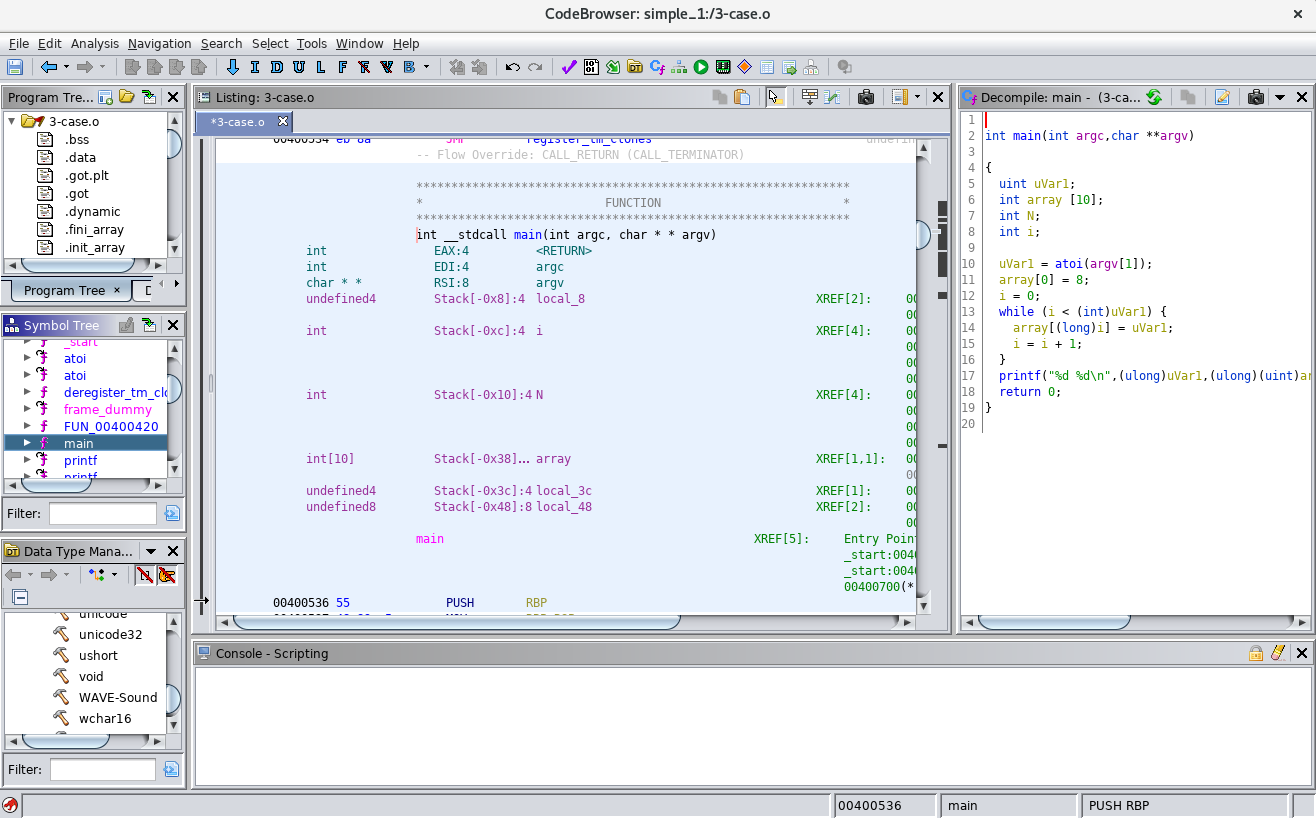
\includegraphics[width=165mm]{images/ghidra.png}
\caption{Ghidra - Graphical User Interface\label{fig:fig24}}
\end{figure}

\chapter{Implementation}

The goal of this work is to ensure the security of binaries from memory safety violations. In particular, our work is focused on adding a spatial memory safety protection, as discussed before. We use Intel's Pin tool interface and NSA's Ghidra interface to implement our technique. Intel's Pin tool provides an application programming interface (API) to analyze the binary using dynamic instrumentation. National Security Agency's (NSA) Ghidra is a reverse engineering framework, which also provides an extensive application programming interface (API). Our implementation consists of two parts. One of them is the "Pintool", built in \texttt{C++} using Intel Pin framework, which is used to add run time checks using dynamic binary instrumentation techniques. This tool keeps bounds information per pointer/array in a structure and add validity checks according to accesses. Pintool takes an input that is statically generated by using Ghidra interface. This script is the other part of our technique. This script analyses the binary, that is compiled using \texttt{gcc} debug flag (thus keeping debugging information) and fetches the required information by reverse engineering the binary (which is then fed to the Pintool). We assume that the source code is not available for us to analyze, and our implementation only considers the symbol information from the binary (compiled using gcc debug flag) for the analysis (this information makes the analysis better). The remaining chapter talks about our implementation in details.

\section{Script Using Ghidra API}
First part of our implementation is this Ghidra script, which gets the information from the \texttt{elf} binary compiled using \texttt{gcc} debug flag \texttt{-g}. This flag retains the symbol or debugging information in the executable in the form of \texttt{dwarf} (debugging with attribute record formats \citep{eager2007introduction}) format (We assume that the binaries to be protected are pre-compiled in this way, so that they retain the debugging information, which improves the precision of static analysis done by Ghidra). As described before, Ghidra can be run in GUI (graphical user interface) or in CLI (command line) mode. Ghidra is being shipped with \texttt{analyzeHeadless} tool (shell script), which can be used to run Ghidra in the command line mode. Ghidra comes with a rich API, which can be used to write scripts in \texttt{Java} or in \texttt{Python 2.7}, to analyze the information generated by reverse engineering the executable. Our implementation uses \texttt{Python 2.7} for convenience and simplicity.

\begin{figure}
\begin{centering}
\begin{tabular}{ c | c }
\begin{lstlisting}
for(int i=0 ; i<N ; i++)
    array[i] = N;
\end{lstlisting}
&
\begin{lstlisting}
4004a8 jmp 4004ba <main+0x24>
4004aa mov eax,DWORD PTR [rbp-0x4]
4004ad cdqe
4004af mov edx,DWORD PTR [rbp-0x8]
4004b2 mov DWORD PTR [rbp+rax*4-0x30],edx
4004b6 add DWORD PTR [rbp-0x4],0x1
4004ba mov eax,DWORD PTR [rbp-0x4]
4004bd cmp eax,DWORD PTR [rbp-0x8]
4004c0 jl 4004aa <main+0x14>
\end{lstlisting}
\end{tabular}
\caption{Array Stores Using A For Loop\label{fig:fig31}}
\par\end{centering}
\end{figure}

The Ghidra script fetches all the local (i.e. variables present on stack) and global (i.e. the variables in data and/or bss section) variables, their details and the important assembly instructions related to their use (access instructions). For example, consider a part of \texttt{C} code and corresponding \texttt{x86-64 assembly} instructions for that part in \cref{fig:fig31}. As seen from this example, it is clear that the destination operand in the instruction at the location \texttt{4004b2} belongs to an array \texttt{array[]}. Hench, we mark the "instruction owner" of the instruction at \texttt{4004b2} as \texttt{array[]}. Consider another example in \cref{fig:fig32}. In this case, the instruction at \texttt{40049a} belongs to array \texttt{b}, the instruction at \texttt{4004a5} belongs to the pointer \texttt{ptr}, and the instruction at \texttt{4004b0} belongs to the scalar \texttt{c}, based on the addresses (relative to the base pointer) in the destination operand. Now, consider the code \texttt{c = *(ptr + 10);} in \texttt{C}, assembly instructions from the location \texttt{4004a9} to \texttt{4004b0} represent that part. Here, the pointer \texttt{ptr} is overflowing the array \texttt{b}, and hence we should check the source operands of the instructions to determine the invalid accesses. Notice that the pointer is being moved to the register \texttt{rax} at location \texttt{4004a9} and then after some arithmetic, there is an invalid access of the pointer at the location \texttt{4004ad}. To catch such invalid accesses, we have implemented a analysis algorithm, which keeps track of the registers (the register in which the pointer address is first copied, in this case, location \texttt{4004a9}) and contains this pointer location value (note that the value of the pointer location present in register \texttt{rax} can be moved to (say) register \texttt{rcx}, which then can be used to overflow the array). Then, it checks for all the register loads of the registers containing the pointer location. Thus, in this case, the "instruction owner" of the instruction at \texttt{4004ad} is determined as the pointer \texttt{ptr}. "Instruction owner" is nothing but the variable defined in \texttt{C} code.

\cref{fig:fig33} shows the output of Ghidra script (including comments) after analysing the example program shown in \cref{fig:fig32}. The output is in text format and is fed to the PIN tool. This output file from the Ghidra script contains addresses mapped to their "instruction owners" (listed under "addresses") (these addresses determine which instructions are to be analysed), function local variables (listed under "locals"), static variables (these go in the data or bss sections and defined under the function name-spaces) (listed under "namespace") and global variables (these go in the data or bss sections and defined under the global name-space) (listed under ".global"). Note that the "instruction owner" is nothing but the variable, which is related to the specific instruction, according to our technique as explained before. Ghidra determines the variable names using debugging (symbol) information, or it assigns random names, if the debugging (symbol) information is not available. Local variables (or "instruction owners") are associated with the metadata, like owner name (stored as functionname\_variablename format if local to a function or .global\_variable format if defined globally), position on the stack relative to rbp, size and owner type. Variables (or instruction owners) defined in the "data" or "bss" are associated with their static address, instead of position on the stack relative to rbp and rest of the metadata is same. This example has no static variables defined which are local to the function (hence, nothing is listed under "namespace"). Also, notice the pointer \texttt{global\_PTR\_\_\_gmon\_start\_\_\_00600ff} listed under ".global", it is a symbol produced by Ghidra API and is a false positive. But, it would not affect our implementation, as it has not been accessed anywhere in the code. Removing such false positives is left for the future work. Also, we store local variables in functionname\_variablename format and global variables .global\_variable format, just to distinguish between same variable names across functions and global scope. Note that Ghidra assigns different names to the variables defined inside the same function but with different local scopes. For e.g. for the following code:

\begin{lstlisting}
int main()
{
  {
    int c;
    c = 8;
  }
  int c = 5;
  return 0;
}
\end{lstlisting}
Ghidra distinguishes between different "\texttt{c}"s, by inferring them as \texttt{c} and \texttt{c\_1}. Hence, we don't have to set naming conventions to distinguish between those two.

\begin{figure}
\begin{centering}
\begin{tabular}{ c | c }
\begin{lstlisting}
int main()
{
  int b[5];
  b[0] = 1;
  int *ptr = b;
  int c = *(ptr + 10);
  return 0;
}
\end{lstlisting}
&
\begin{lstlisting}
400496 push rbp
400497 mov rbp,rsp
40049a mov DWORD PTR [rbp-0x20],0x1
4004a1 lea rax,[rbp-0x20]
4004a5 mov QWORD PTR [rbp-0x8],rax
4004a9 mov rax,QWORD PTR [rbp-0x8]
4004ad mov eax,DWORD PTR [rax+0x28]
4004b0 mov DWORD PTR [rbp-0xc],eax
4004b3 mov eax,0x0
4004b8 pop rbp
4004b9 ret
\end{lstlisting}
\end{tabular}
\caption{Invalid Pointer Access\label{fig:fig32}}
\par\end{centering}
\end{figure}

\begin{figure}
\begin{centering}
\begin{lstlisting}
1           // Number of functions
main        // Function name

addresses   // Function addresses and instruction owner information
40049a main_b
4004a1 main_b
4004b0 main_c
4004a5 main_ptr
4004ad main_ptr

locals      // Function local variables
-32 array main_b 20
-12 scalar main_c 4
-8 pointer main_ptr 8

namespace   // Static variables local to the function

.global     // Global variables
6295544 pointer .global_PTR___gmon_start___00600ff8 8
\end{lstlisting}
\caption{Output of Ghidra tool after analysing the code in \cref{fig:fig32}\label{fig:fig33}}
\par\end{centering}
\end{figure}

\section{Pintool}
As mentioned before, this tool is one of the important parts of our implementation. We use this to detect the actual spatial memory safety violations i.e. the overflow attacks, using dynamic instrumentation. Static binary information generated using our Ghidra script is fed to the Pintool, to determine dynamic checks for possible variables according to their access instructions in the assembly code. First, the Pin tool associates instruction address to their instruction owners and stores them in a map structure (which stores instruction address as a key and an object containing corresponding instruction owner metadata as a value). Because of the map structure, it becomes easier and quicker to access the instruction owner and other metadata during instruction instrumentation. Bounds information is stored per instruction owner in a global map structure. The idea is to create a structure, that is similar to that used by the SoftBound technique. This structure stores the base and bounds of each instruction owner, which can be used to validate accesses when needed. Base and bound are the actual locations on the memory. Base is the base pointer at the location of the assigned object and bound is base pointer plus size of the object. We categorize the instruction owners as scalar, array and pointer. But, validation checks are not added for scalar loads and stores as it is redundant.

Image and instruction instrumentation is used to implement the detection mechanism. Image instrumentation is required to add instrumentation for routines (for e.g. Malloc, Calloc,etc.) and instruction instrumentation is required to add instrumentation for instructions which are mapped with corresponding instruction owners as shown in \cref{fig:fig33}. Now, consider the code in \cref{fig:fig32}, it is an example of invalid pointer access (out of bounds of the allocated object). \cref{fig:fig34} shows points at which the checks get added in assembly, which can be visualized as the corresponding checks in the source code. Checks are nothing but analysis routines called by instruction instrumentation routine. Notice that the instruction addresses detected by Ghidra (\cref{fig:fig33}) are 5 in total and we have added only 3 checks. The reason is that we ignore instructions with \texttt{lea} opcode (load effective address) (instruction at \texttt{4004a1}) and instructions related to scalar loads and stores (instruction at \texttt{4004b0}), as they are not required for our implementation. Using Pin API, checks can be added before and after the instruction once it has been detected by the instruction instrumentation routine. In this case, checks are added just before the instructions to be analyzed (in this case - \texttt{40049a}, \texttt{4004a5} and \texttt{4004ad}) to prevent the invalid access. As the execution starts the first instruction detected is the instruction at \texttt{40049a}. Pintool adds an analysis routine just before the instruction. First, the routine detects its instruction owner by querying the hash map using instruction address (\texttt{40049a}) (which returns an object containing the owner metadata). Second, it checks if the owner name is present in the global map structure (and hence owners are renamed by function\_variablename or .global\_variablename convention, as described before) which contains bounds information. If not, it calculates the bounds (using instruction owner metadata) and adds the bounds information into the global map, with owner as a key. The calculation is as follows:
\begin{lstlisting}
        |---->  lower_bound = rbp - 32
main_b  |
        |---->  upper_bound = rbp - 32 + size = rbp - 32 + 19
\end{lstlisting}
Note that all the values are in decimal. As this is the first occurrence of \texttt{main\_b}, the bound information is added into the global map. Third, it checks if the access is within the bounds as follows:
\begin{lstlisting}
if (access < lower_bound || access > upper_bound)
    abort;
\end{lstlisting}
In this case, access is \texttt{rbp - 32} (which is nothing but \texttt{rbp - 0x20} in hex). Note that, in this case the address is relative to rbp, but this may not be true in other cases. For example, in case of malloc, the addresses are stored on heap and in case of static variables \texttt{rip} relative addressing is used, unlike rbp relative addressing in case of local variables. Hence, in those cases the bounds checks would be similar, but bound calculation changes. The bound calculation in the case of variables in data section is as follows:
\begin{lstlisting}
            |---->  lower_bound = address
main_owner  |
            |---->  upper_bound = address + size
\end{lstlisting}
Here, address is the static address of the variable. This is the reason why, in case of static or global variables, we store static address in the metadata, unlike relative to rbp in case of local variables, as described before. Back to our example - after the bounds check, the execution moves on to the next instruction (\texttt{4004a5}). Here, pointer \texttt{ptr} is being assigned the address of \texttt{b} (tool does this, by finding the contents of the register, which is the address of an array). Hence, \texttt{ptr} acquires the bounds of array \texttt{b}. This is similar to the pointer assignment in SoftBound.

SoftBound supports pointer metadata propagation, i.e. it propagates the pointer bounds information whenever pointers are passed to a different function. SoftBound transforms the function in such a way that, it passes the bounds information as function arguments. Our implementation also supports transfers or propagation of the bounds information, similar to the SoftBound approach but by using a different strategy. It does this in the following way. Figure \cref{fig:fig35} presents the bounds propagation technique. In the function "main", the location of array \texttt{b} is moved in the register \texttt{rdi} (instruction at \texttt{4004c6}) and the function foo gets called. Then, in the function foo, the value of \texttt{rdi} (which is nothing but the location of array \texttt{b}) is assigned to the pointer \texttt{ptr} (instruction at \texttt{40049a}) (Note that, according to x86-64 - linux calling convention first six arguments are passed through registers and rest of them are pushed on the stack). Hence, pointer \texttt{ptr} acquires the bounds of array \texttt{b}. Next, pointer \texttt{ptr} is assigned to pointer \texttt{x} (at instruction \texttt{4004a2}) and \texttt{x} acquires the bounds of pointer \texttt{ptr} and thus eventually acquiring the bounds of array \texttt{b}. Pointer \texttt{x} is then used to overflow the assigned object (instruction at \texttt{4004aa}). Hence, a validity check can be added there. It is to be noted that our implementation doesn't support pointer bounds narrowing, but we keep it as a future work. Above discussed implementation details can be visualized from \cref{fig:fig36}.
\begin{figure}
\begin{centering}
\begin{tabular}{ c | c }
\begin{lstlisting}
int main()
{
  int b[5];
  // Check-1
  b[0] = 1;
  // Check-2
  int *ptr = b;
  // Check-3
  int c = *(ptr + 10);
  return 0;
}
\end{lstlisting}
&
\begin{lstlisting}
400496 push rbp
400497 mov rbp,rsp
// Check-1 //
40049a mov DWORD PTR [rbp-0x20],0x1
4004a1 lea rax,[rbp-0x20]
// Check-2 //
4004a5 mov QWORD PTR [rbp-0x8],rax
4004a9 mov rax,QWORD PTR [rbp-0x8]
// Check-3 //
4004ad mov eax,DWORD PTR [rax+0x28]
4004b0 mov DWORD PTR [rbp-0xc],eax
4004b3 mov eax,0x0
4004b8 pop rbp
4004b9 ret
\end{lstlisting}
\end{tabular}
\caption{Invalid Pointer Access (with checks)\label{fig:fig34}}
\par\end{centering}
\end{figure}

\begin{figure}
\begin{centering}
\begin{tabular}{ c | c }
\begin{lstlisting}
void foo(int *ptr)
{
  int* x = ptr;
  int y = *(x+5);
}

int main()
{
  int b[5];
  b[0] = 1;
  foo(b);
  return 0;
}
\end{lstlisting}
&
\begin{lstlisting}
<foo>:
400496 push rbp
400497 mov rbp,rsp
40049a mov QWORD PTR [rbp-0x18],rdi
40049e mov rax,QWORD PTR [rbp-0x18]
4004a2 mov QWORD PTR [rbp-0x8],rax
4004a6 mov rax,QWORD PTR [rbp-0x8]
4004aa mov eax,DWORD PTR [rax+0x14]
4004ad mov DWORD PTR [rbp-0xc],eax
4004b0 nop
4004b1 pop rbp
4004b2 ret

<main>:
4004b3 push rbp
4004b4 mov rbp,rsp
4004b7 sub rsp,0x20
4004bb mov DWORD PTR [rbp-0x20],0x1
4004c2 lea rax,[rbp-0x20]
4004c6 mov rdi,rax
4004c9 call 400496 <foo>
4004ce mov eax,0x0
4004d3 leave
4004d4 ret
\end{lstlisting}
\end{tabular}
\caption{Bounds propagation\label{fig:fig35}}
\par\end{centering}
\end{figure}

\begin{figure}
\begin{centering}
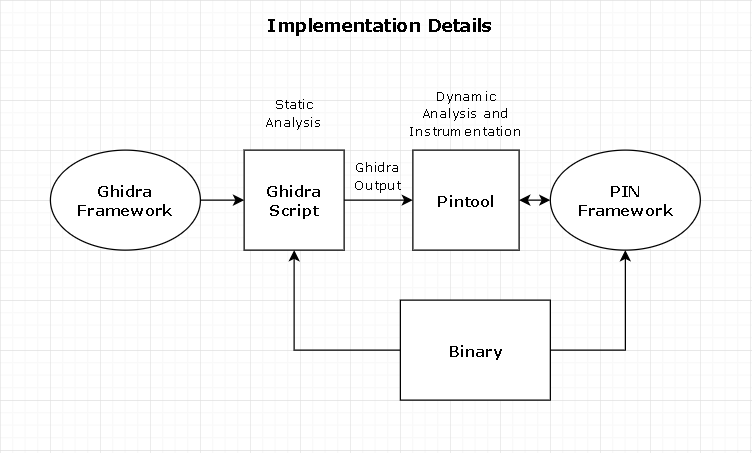
\includegraphics[width=138mm]{images/implementation_details.png}
\caption{Implementation Details\label{fig:fig36}}
\par\end{centering}
\end{figure}

\chapter{Experiments}
In this section, we describe the implementation details and the experimental results obtained after running the benchmark tests. This helps us evaluating the effectiveness of this technique.

\section{Experimental Setup}
All the experiments are performed on a 64-bit Intel Xeon processor with little-endian architecture and x86 instruction set. Fedora 28 is used as an operating system with kernal version 5.0.9-100.fc28.x86\_64. It is to be noted that Java is needed to install the Ghidra software as shown in the documentation \citep{ghidrainstallation}. Ghidra script is written using python and GNU compiler collection is required for running PIN software, designing the Pintool and for the benchmark suite. The implementation details with version information are shown in \cref{tab:table41}.\\
\begin{table}[ht]
\centering\small
\begin{tabularx}{\linewidth}{lX}
\toprule
Tool & Version Details\\
\midrule
Operating System & Fedora release 28\\
Kernel version & 5.0.9-100.fc28.x86\_64\\
GNU compiler collection (gcc and g++) & 8.3.1\\
Intel PIN & pin-3.7-97619-0d0c92f4f\\
Ghidra & 9.0.3-DEV\\
Java JDK & 11.0.2\\
Python & 2.7\\
\bottomrule
\end{tabularx}
\caption{Implementation Details\label{tab:table41}}
\end{table}

To test our implementation, we used SARD - 81 and SARD - 89 test suites (Refer - \citep{black2017sard} \citep{sardcite}) and our own test cases. SARD - 81 has 5 cases and all of them are with buffer overflows. SARD - 89 suite has 291 cases, each having a combination of tests with and without buffer overflows (1164 cases in total). These test cases manifests the vulnerabilities including CWE-119 \citep{cwe119} and CWE-121 \citep{cwe121}. CWE-119 being the top weakness in the "2019 CWE Top 25 Most Dangerous Software Errors"\citep{2019cwetop25} list. We have also created about 50 test cases with overflows, but we do not include those in the results, as those test cases are not standardized. SARD cases consist of buffer overflows with and without using library functions. Note that these test cases only consist of \texttt{C} programs.

\section{Overflow Detection}
In this section, we will discuss about the detection effectiveness of our technique. The end goal of this work is to detect all kinds of memory errors, including spatial memory errors and temporal memory errors. Currently, our technique is focused on providing spatial safety, as discussed earlier. We tested our implementation using SARD benchmarks as discussed before. In case of SARD - 81 benchmark suit, 2 out of 5 tests are passed and in case of SARD - 89 suit, 664 out of 1164 tests are passed. This can be visualized from figures \cref{fig:fig41} and \cref{fig:fig42}. Hence, about 57\% test cases are passed. It should be recalled that all the test cases in SARD - 81 suit show buffer overflows, but SARD - 89 has a combination of tests with and without buffer overflows. 291 of 1169 (i.e. 5 from SARD - 81 and 1164 from SARD - 89) test cases are without overflows. The cases with buffer overflow include overflow by small, medium and large quantity. Also, these cases consist of buffer overflows using library functions, for e.g. using malloc and without using library functions, for e.g. using arrays.

\begin{table}[ht]
\centering\small
\begin{tabularx}{\linewidth}{lX}
\toprule
Reason & Number of Test Cases\\
\midrule
Ghidra script failed to detect & 446\\
Pintool failed to detect & 9\\
String copy (strcpy and strncpy) functions & 25\\
Shared memory Operation (shmat) function & 4\\
Get current working directory (getcwd) function & 3\\
Copy memory area (memcpy) function  & 12\\
Threading & 4\\
\bottomrule
\end{tabularx}
\caption{Case Failure Details (SARD - 81 and SARD - 89)\label{tab:table42}}
\end{table}

\begin{figure}
\begin{centering}
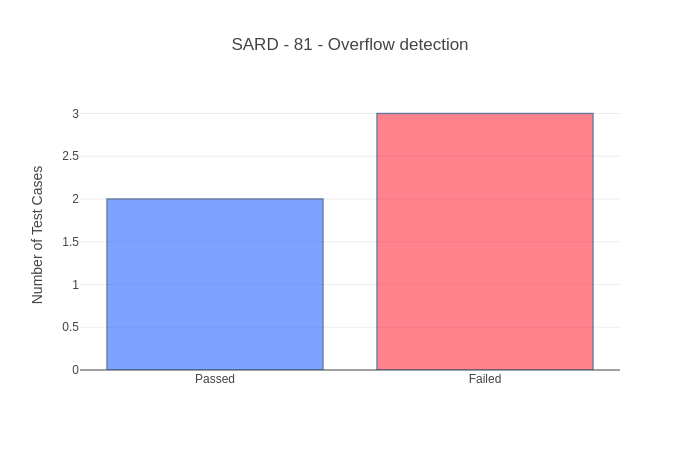
\includegraphics[width=140mm]{images/sard81.png}
\caption{Overflow Detection - SARD - 81\label{fig:fig41}}
\par\end{centering}
\end{figure}

\begin{figure}
\begin{centering}
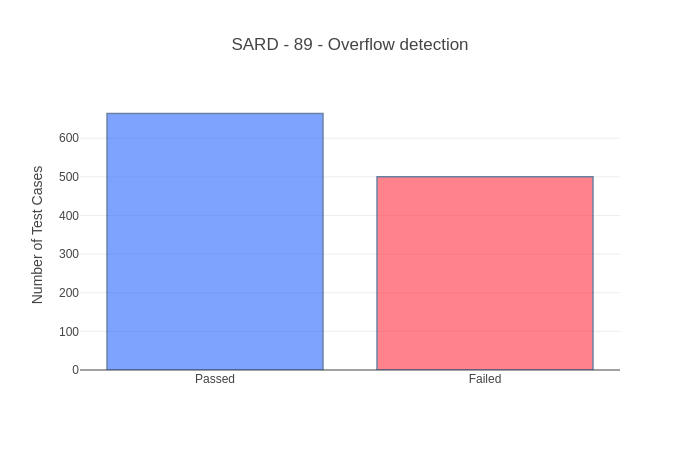
\includegraphics[width=140mm]{images/sard89.png}
\caption{Overflow Detection - SARD - 89\label{fig:fig42}}
\par\end{centering}
\end{figure}

\cref{tab:table42} shows reasons of case failures and the number of failed cases per reason for both SARD - 81 and SARD - 89 benchmarks (i.e. considering 1169 cases in total). Overflows using library functions such as strcpy, strncpy, shmat, getcwd, memcpy are undetected, as library functions are not currently supported (although we manually detect malloc, calloc, realloc, fgets, gets and free). Multi threading is not yet supported and we keep this as a future work. Pintool failed to detect 9 of the cases. This is because certain instructions or pattern of instructions are not being analysed by our Pintool and this can be avoided by carefully modifying the algorithm for those particular cases and other edge cases that may occur. Lastly, there are 446 cases - a significant amount of cases, that are not detected by Ghidra script (Note that these cases may contain library functions, but there may not be a direct impact of library functions on the detection mechanism). The reasons for that include:
\begin{itemize}
    \item \textbf{The location of array access instruction is not detected.}
    \item \textbf{The location of array access instruction is detected incorrectly.}
    \item \textbf{The owner is not detected.}
    \item \textbf{The owner size is detected incorrectly.}
\end{itemize}
The problems in detecting locations of array accesses occur primarily ("primarily", because we observed this in most of the cases) because Ghidra framework's internal algorithms failed to determine it. This may also happen if our algorithm fails to conduct further analysis at run time. For e.g. consider a \texttt{c} program and corresponding assembly in \cref{fig:fig43}. Looking only at the assembly code, it is difficult to predict if the instruction at location \texttt{4004ee} belongs to array \texttt{b1} or if it belongs to array \texttt{b2}. As seen from the example code, array \texttt{b2} clearly overflows and hence the code prints 1 as an output. For the above code, Ghidra predicts the owner of the location \texttt{4004ee} incorrectly, as \texttt{b1} (i.e. it predicts incorrect instruction owner, consequently affecting our technique). \cref{fig:fig44} gives actual examples from SARD benchmarks (Refer - \citep{black2017sard} \citep{sardcite}), which fail to detect the array access instructions. In the program on the left, the array access instruction is falsely predicted as accessed by a scalar and not by an array (and thus the existence of scalar in the code is predicted falsely). In the program on the right, the array access instruction is not detected and hence no owner is assigned to this instruction, which leads to overflow detection failure. We also observed that the access location is mostly detected if the array is indexed using a variable. The chances of detecting the access locations of overflowed arrays become dimmer if the they are indexed using raw numbers (the ones that overflow). As most of cases in SARD suits are close to the ones shown in \cref{fig:fig44}, the failure percentage is higher than expected. \cref{fig:fig44}, \cref{fig:fig45}, \cref{fig:fig46}, \cref{fig:fig47}, \cref{fig:fig48}, \cref{fig:fig49} and \cref{fig:fig410} show examples of each of the above discussed cases (actual examples from SARD benchmarks (Refer - \citep{black2017sard} \citep{sardcite})).

\begin{figure}
\begin{centering}
\begin{tabular}{ c | c }
\begin{lstlisting}
#include <stdio.h>
int main()
{
  int b1[5];
  int b2[10];
  b2[15] = 1;
  printf("%i\n", b1[3]);
  return 0;
}
\end{lstlisting}
&
\begin{lstlisting}
4004e6 push rbp
4004e7 mov rbp,rsp
4004ea sub rsp,0x50
4004ee mov DWORD PTR [rbp-0x14],0x1
4004f5 mov eax,DWORD PTR [rbp-0x14]
4004f8 mov esi,eax
4004fa mov edi,0x400590
4004ff mov eax,0x0
400504 call 4003f0 <printf@plt>
400509 mov eax,0x0
40050e leave
40050f ret 
\end{lstlisting}
\end{tabular}
\caption{Ambiguous Array Access\label{fig:fig43}}
\par\end{centering}
\end{figure}

\begin{figure}
\begin{centering}
\begin{tabular}{ c | c }
\begin{lstlisting}
int main(int argc, char *argv[])
{
  char buf[10];
  /*  BAD  */
  buf[10] = 'A';
  return 0;
}
\end{lstlisting}
&
\begin{lstlisting}
int main(int argc, char *argv[])
{
  char buf[10];
  /*  BAD  */
  buf[4105] = 'A';
  return 0;
}
\end{lstlisting}
\end{tabular}
\caption{Ghidra Script detection failure (example is Taken from SARD suit~\protect\citep{sardcite})\label{fig:fig44}}
\par\end{centering}
\end{figure}

\begin{figure}
\begin{centering}
\begin{tabular}{ c }
\begin{lstlisting}
int main(int argc, char *argv[])
{
  int i;
  char buf[10];
  i = 9;
  /*  OK  */
  (buf + i)[0] = 'A';
  return 0;
}
\end{lstlisting}
\end{tabular}
\caption{Pintool detection failure (example is Taken from SARD suit~\protect\citep{sardcite})\label{fig:fig45}}
\par\end{centering}
\end{figure}

\begin{figure}
\begin{centering}
\begin{tabular}{ c }
\begin{lstlisting}
#include <string.h>
int main(int argc, char *argv[])
{
  char buf[10];
  /*  BAD  */
  strcpy(buf, "AAAAAAAAAAAAAAAAA");
  return 0;
}
\end{lstlisting}
\end{tabular}
\caption{String Copy (strcpy) (example is Taken from SARD suit~\protect\citep{sardcite})\label{fig:fig46}}
\par\end{centering}
\end{figure}

\begin{figure}
\begin{centering}
\begin{tabular}{ c }
\begin{lstlisting}
#include <sys/types.h>
#include <sys/ipc.h>
#include <sys/shm.h>
#include <assert.h>
#include <stdlib.h>
int getSharedMem()
{
  return (shmget(IPC_PRIVATE, 10, 0xffffffff));
}
void relSharedMem(int memID)
{
  struct shmid_ds temp;
  shmctl(memID, IPC_RMID, &temp);
}
int main(int argc, char *argv[])
{
  int memIdent;
  char * buf;
  memIdent = getSharedMem();
  assert(memIdent != -1);
  buf = ((char *) shmat(memIdent, NULL, 0));
  assert(((int)buf) != -1);
  /*  BAD  */
  buf[17] = 'A';
  shmdt((void *)buf);
  relSharedMem(memIdent);
  return 0;
}
\end{lstlisting}
\end{tabular}
\caption{Shared Memory Operations (shmat) (example is Taken from SARD suit~\protect\citep{sardcite})\label{fig:fig47}}
\par\end{centering}
\end{figure}

\begin{figure}
\begin{centering}
\begin{tabular}{ c }
\begin{lstlisting}
#include <unistd.h>
int main(int argc, char *argv[])
{
  char buf[10];
  /*  BAD  */
  getcwd(buf, 18);
  return 0;
}
\end{lstlisting}
\end{tabular}
\caption{Current working directory (getcwd) (example is Taken from SARD suit~\protect\citep{sardcite})\label{fig:fig48}}
\par\end{centering}
\end{figure}

\begin{figure}
\begin{centering}
\begin{tabular}{ c }
\begin{lstlisting}
#include <string.h>
int main(int argc, char *argv[])
{
  int copy_size;
  char src[4106];
  char buf[10];
  memset(src, 'A', 4106);
  src[4106 - 1] = '\0';
  copy_size = -1;
  if (copy_size <= (int)(sizeof buf))
  {
    /*  BAD  */
    memcpy(buf, src, copy_size);
  }
  return 0;
}
\end{lstlisting}
\end{tabular}
\caption{Copy memory area (memcpy) (example is Taken from SARD suit~\protect\citep{sardcite})\label{fig:fig49}}
\par\end{centering}
\end{figure}

\begin{figure}
\begin{centering}
\begin{tabular}{ c }
\begin{lstlisting}
#include <pthread.h>
void * thread_function1(void * arg1)
{
  char buf[10];
  /*  BAD  */
  buf[4105] = 'A';
  pthread_exit((void *)NULL);
  return 0;
}
int main(int argc, char *argv[])
{
  pthread_t  thread1;
  pthread_create(&thread1, NULL, &thread_function1, (void *)NULL);
  pthread_exit((void *)NULL);
  return 0;
}
\end{lstlisting}
\end{tabular}
\caption{Threading (pthread) (example is Taken from SARD suit~\protect\citep{sardcite})\label{fig:fig410}}
\par\end{centering}
\end{figure}

\section{Run Time Overhead}
The run time overhead is also one of the important factors to determine the effectiveness of the mechanism. We used same benchmark suits (SARD) as mentioned in the previous section, to measure the overhead. \cref{fig:fig411} and \cref{fig:fig412} show overhead analysis of SARD - 81 and SARD - 89 suits (\cref{fig:fig413} shows the zoomed in version of \cref{fig:fig412}). We divide the analysis into 3 different tests - test1, test2 and test3. Where test1 calculates the time taken by raw binary to run (i.e. without any tool), test2 calculates the run time of binary if run using a minimal Pintool (a tool with no instrumentation - \cref{fig:fig415}) and test3 computes the time taken by binary if run using our Pintool. We run each test (test1, test2 and test3) 15 times on all the benchmark cases and took the average of those 15 runs for each case. From \cref{fig:fig411} and \cref{fig:fig412} it can be seen that our tool adds a big amount overhead, although considering the minimal tool's overhead, it can be concluded that significant amount of this overhead incurred by pin framework itself (i.e. PIN startup overhead). \cref{fig:fig414} shows average overhead of the 3 tests. Considering the average overheads, we observed about large overhead, but most of the overhead is PIN startup overhead. It will have a negligible effect if measured against bigger programs, as PIN uses code cache, it doesn't have to translate the frequently executing code. By comparing run times of our implementation and the minimal Pintool example, it can be inferred that our implementation adds about 6.15\% overhead. This is due to the inclusion of instrumentation routines in our tool, unlike the minimal Pintool.

\begin{figure}
\begin{centering}
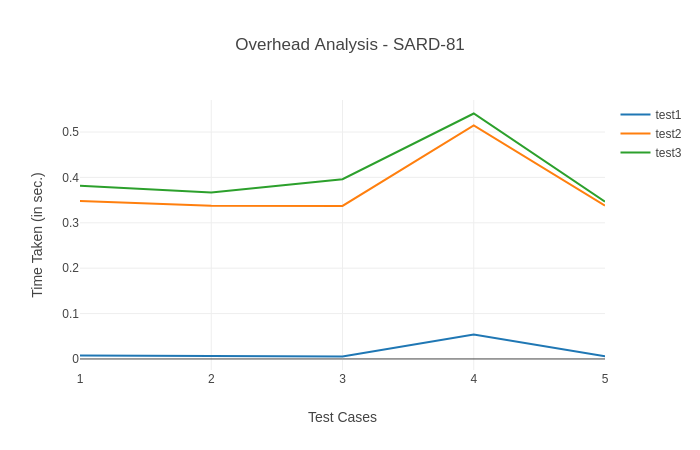
\includegraphics[width=140mm]{images/sard81_overhead.png}
\caption{Overhead Analysis - SARD - 81\label{fig:fig411}}
\par\end{centering}
\end{figure}

\begin{figure}
\begin{centering}
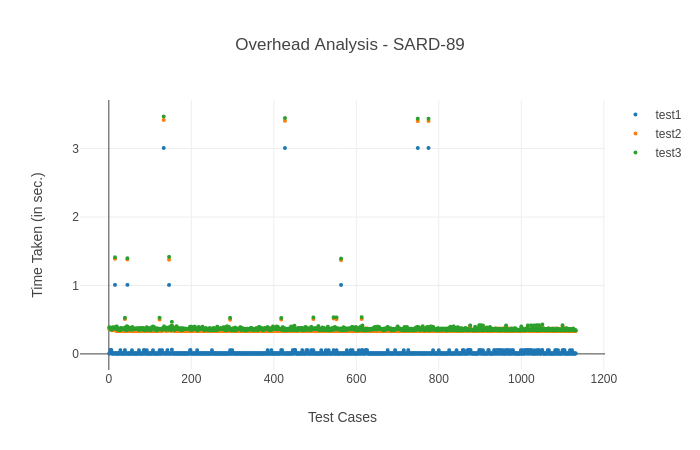
\includegraphics[width=140mm]{images/sard89_overhead.png}
\caption{Overhead Analysis - SARD - 89\label{fig:fig412}}
\par\end{centering}
\end{figure}

\begin{figure}
\begin{centering}
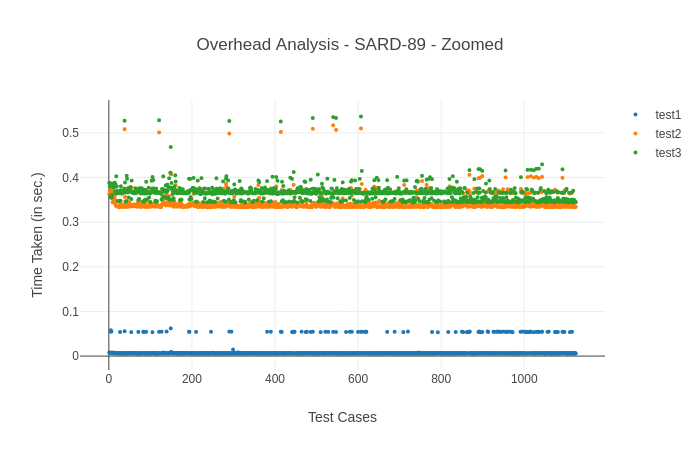
\includegraphics[width=140mm]{images/sard89_overhead_zoomed.png}
\caption{Overhead Analysis - SARD - 89 (zoomed)\label{fig:fig413}}
\par\end{centering}
\end{figure}

\begin{figure}
\begin{centering}
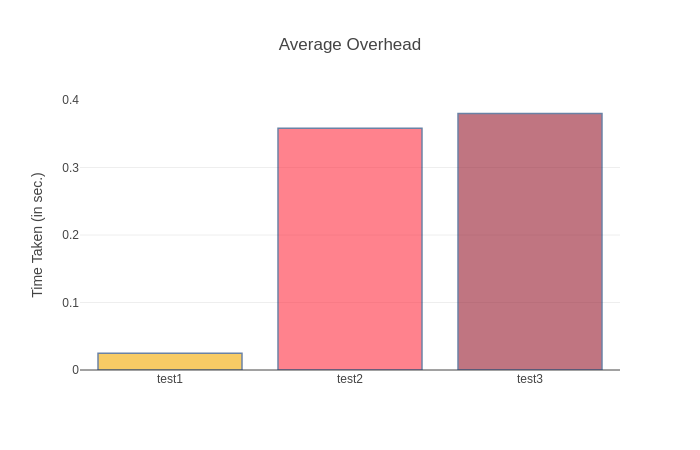
\includegraphics[width=140mm]{images/average_overhead.png}
\caption{Average Overhead\label{fig:fig414}}
\par\end{centering}
\end{figure}

\begin{figure}
\begin{centering}
\begin{tabular}{ c }
\begin{lstlisting}
#include "pin.H"
int main(int argc, char * argv[])
{
    // Initialize pin
    PIN_Init(argc, argv);

    // Start the program, never returns
    PIN_StartProgram();

    return 0;
}
\end{lstlisting}
\end{tabular}
\caption{Minimal Pintool\label{fig:fig415}}
\par\end{centering}
\end{figure}

\chapter{Related and Future Work}

This section discusses the work which has been done in the past, which is related to the goal of this work. This is not limited to the similar techniques used, but also includes a broad overview of memory safety techniques in general. This section also discusses the future work to be done to improve the effectiveness of this technique.

\section{Related Work}

Memory safety violations is one of the oldest issues in programming and computing. These violations occur due to lack of memory safety in languages like \texttt{C} and \texttt{C++}. Buffer overflow vulnerabilities get popularity when Morris Worm \citep{Spafford:1989:IWP:66093.66095} is introduced in 1988 and the overflow attacks are still relevant till this date. There are a number of defences have been proposed to defend against memory attacks (like buffer overflow), for e.g. stack canaries, ASLR, non executable memory, PIE (position Independent Executable), re-randomization techniques, etc. make the attack using buffer overflow very difficult. But, even combination of these defenses can still be circumvented.

Laszlo Szekeres et al. \citep{6547101} explain the type of attacks and the phases in which these attacks can be exploited, memory safety being first and one of the important phases. To provide complete memory safety, spatial as well as temporal memory safety should be provided. In this section, we will only consider the work related to provide protection against memory safety attacks. Numerous approaches have been proposed to provide memory safety against vulnerabilities in low level languages. Memory safety approaches can be categorized as object based, pointer based and tripwire approaches. Now, we look at some of the popular spatial and complete memory safety approaches.

\subsection{Work Focused On Providing Spatial Safety (Primarily)}

Richard W. M. Jones and Paul H. J. Kelly \citep{jones1997backwards} propose a compiler based technique, which does pointer and array bounds checking, without changing pointer representation. Dhujrati et al. \citep{dhurjati2006backwards} propose an improved version of Kelly's technique. They use a technique called automatic pool allocation \citep{lattner2005automatic}, which is based on memory partitioning. SAFECode \citep{dhurjati2006safecode} is another object based approach (improved version of their previous work). It guarantees some from of spatial and temporal safety. CCured \citep{Necula:2002:CTR:565816.503286} ensures type safety in \texttt{C} programs by categorizing pointers into different types (safe pointer, sequence pointer and dynamic pointer) and adding the checks accordingly, either during compile time or during run time. Hence, to keep pointer metadata, it needs to extend the pointer structure (fat pointers). It requires to convert \texttt{C} program into CCured representation and thus it relies on source code. Ruwase et al. proposes a compiler based technique called CRED \citep{ruwase2004practical} which dynamically detects the buffer overflows. Baggy bounds checking \citep{akritidis2009baggy} is an object based technique, which utilizes allocation bounds instead of object bounds. Light weight bounds checking or LBC \citep{Hasabnis:2012:LBC:2259016.2259034} is another spatial memory error detection technique, which provides better performance than the Baggy Bounds checking technique. Hardbound \citep{devietti2008hardbound} is a combination of software and hardware techniques which ensures complete spatial safety. In this approach, the software (compiler or run-time system) allocates pointer bounds and the hardware checks for valid pointer accesses and propagates bounds metadata if necessary. SoftBound \citep{nagarakatte2009softbound} is a compiler based technique which enforces complete spatial safety, without any hardware support. The basic idea of our work is based on SoftBound approach, as explained before. AddressSanitizer \citep{serebryany2012addresssanitizer} is a trip-wire technique which detects buffer overflows and use-after-free errors. Code-pointer integrity \citep{kuznetsov2014code} prototype enforces spatial safety, though it is primarily made to defend against control flow hijack attacks. Intel MPX \citep{oleksenko2017intel} is a recent work by Intel. It provides spatial safety using hardware assistance.

\subsection{Work Focused On Providing Complete Memory Safety}

SafeC \citep{austin1994efficient} is a fat pointer approach, which provides both spatial and temporal safety. Patil et al. \cite{patil1995efficient} propose a memory safety (spatial plus temporal) technique using shadow processor. The idea is to use one processor to execute the program and the other (shadow) to monitor that program. Cyclone \citep{Jim:2002:CSD:647057.713871} is another fat pointer based approach, which is source code dependent. Cyclone is a \texttt{C} dialect which transforms \texttt{C} code in Cyclone code and uses static analysis and/or adds dynamic checks to ensure safety. It also detects temporal memory errors like dangling pointers. Yong et al. \citep{yong2003protecting} propose a memory safety approach using static code analysis and instrumentation techniques. Xu et al. \citep{xu2004efficient} present a memory safety approach which requires source code transformation to add dynamic checks. Watchdog \citep{nagarakatte2012watchdog} and WatchdogLite \citep{nagarakatte2014watchdoglite} ensure spatial and temporal memory safety using hardware assistance. One more approach from Nagarakatte et al. called SoftBoundCETS \citep{nagarakatte2015everything} is focused on providing complete memory safety. It combines SoftBound approach (for spatial safety) and CETS approach (for temporal memory safety) \citep{nagarakatte2010cets} to achieve complete safety. MemSafe \citep{simpson2013memsafe} is a compiler based technique which provides complete memory safety. SHAKTI-MS \citep{Das:2019:SRP:3316482.3326356} is a light-weight processor made to offer spatial and temporal safety in \texttt{C} programs. The idea is store pointer metadata on stack, to remove the need of external table (like shadow table) and to reduce access overhead. There are a number of approaches which are only focused on providing complete temporal safety (and not spatial safety), but we will not cover those approaches here.

\section{Future Work}
In this section, we discuss multiple future research directions and things that need to be improved. We take inspiration from related studies to improve our technique.

\subsection*{Temporal Safety}
The end goal of our work is to provide complete memory safety, but our technique currently focuses on providing spatial safety only. Ensuring temporal safety and eventually providing complete memory safety will be the principle future direction. It is important to provide complete memory safety to make low level languages safe from memory corruption attacks. One way to provide temporal safety is to extend this work on the basis of SoftBoundCETS \citep{nagarakatte2015everything} technique. They use lock and key metadata with pointers along with the pointer bounds metadata. Hence lock, key and bounds information are propagated together. Key is the unique allocation identifier coupled with each memory allocation and lock is the pointer to a memory location. The access is valid if key and the value at the location pointer by lock matches. Key and lock provides temporal safety, while bounds metadata provides spatial safety.

\subsection*{Completeness}
As discussed before in the experiments section, about 57\% test cases are passed and hence about 43\% cases failed. But, most of this cases are failed due to incapability of Ghidra to predict the correct owner access information. Ghidra has just been open sourced and it is still in the process of improvement. Therefore, instead of totally relying on Ghidra algorithm, certain instruction pattern recognition or machine learning techniques can be used to learn the instruction patterns, detect correct owners, accesses and consequently improve the detection algorithm of our script. Completeness is necessary to remove false positives and detect all the true positives that may remain undetected.

\subsection*{Optional Debugging Information}
Our implementation currently requires program to be compiled by keeping the debugging information, i.e. program must be compiled with -g flag (when compiled using gcc). This helps keeping a lot of information from source code (for e.g. exact variable names). Ghidra tool prediction works better given that this information is present. It is not always possible for the developer to compile the program keeping the debugging information, mainly for the reasons such as code privacy, size requirements, etc. and the binary is mostly optimized for performance, security, privacy, size restrictions, etc. reasons. Also, already compiled binaries and binaries from unknown authors restrict the requirement of keeping debugging information. It is interesting to see how much information can be extracted from the binary which does not contain any symbol information or which has been heavily optimized.

\subsection*{Overhead Reduction and SPEC Benchmark Checks}
It can be observed that, our Pintool incurs about 6\% of overhead on top of the overhead incurred by a minimal Pintool. We will use longer running benchmarks from the SPEC suite to assess the overhead compared to a native execution. It is also important to check if any reduction in the overall overhead is possible by tweaking our Pintool program to decrease the instrumentation checks. For e.g. instrumentation can be added only for store instructions to check for possible buffer overrun. If possible, other instrumentation tools can also be considered.

\subsection*{Other Improvements}
Pointer bounds narrowing and arbitrary or guileful type casts check are also important, but we have not taken those into consideration in our work and will be one priority in our future work considerations. Our work is currently limited to x68-64 architecture and have not been implemented for other architectures. To increase the reach of this technique, it can definitely be made to support other architectures.

\chapter{Conclusion}

We propose a novel approach which employs spatial safety in compiled binaries, with no source code support and no changes in compiler or operating system software. Our approach is based on SoftBound technique, which stores bounds metadata per instruction owner. Instruction owner and their access instruction information is predicted by using reverse engineering techniques. Instruction owner is nothing but variable (e.g. pointer) defined in actual source code (determined by reverse engineering). Instrumentation checks are added on every load and store instructions and checks are made based on the bounds information of that instruction owner, which is associated with the instruction. Instruction owner information is determined using static analysis and reverse engineering techniques, and run time checks are added using dynamic instrumentation techniques. We use Ghidra for static analysis and Pin framework to add dynamic instrumentation. Our technique was able to detect about 57\% of test cases with about 6\% overhead on top of minimal Pintool overhead. In future work section, we propose work needed to increase the detection percentage to further improve this technique.

\global\long\def\bibname{References}%

\bibliographystyle{apalike2}
\bibliography{Biblio/allcites}


% \appendix
% 
\chapter{My Appendix, Next to my Spleen}

Yeah, but not yet, I have to complete the rest of the paper first.
\end{document}
